\apendice{Especificación de Requisitos}
En este apartado se procederá a explicar el diseño de requisitos necesario para el desarrollo de este proyecto.

\section{Introducción}
En este apéndice se van a describir los requisitos que definen como el comportamiento con el que se va a construir el sistema del proyecto.
\section{Objetivos generales}
Los objetivos generales del proyecto van a ser:
\begin{itemize}
    \item Desarrollar una \textit{API} funcional conectada a una base de datos dando servicio para gestionar instancias de tipo: 
        \begin{itemize}
            \item \textit{\textbf{Rooms.}}
            \item \textit{\textbf{Tags.}}
            \item \textit{\textbf{Anchors.}}
            \item \textit{\textbf{Users.}}
            \item \textit{\textbf{Artworks.}}
            
        \end{itemize}   
    \item Desarrollar una aplicación web que contenga un mapa mostrando:
        \begin{itemize}
            \item \textbf{\textit{Rooms} dibujadas por los usuarios guía.}
            \item \textbf{\textit{Tags} con su localización \textit{indoor} a tiempo real.}
            \item \textbf{\textit{Anchors} con su localización \textit{indoor} real en el mapa.}
        \end{itemize} 
    \item Dar acceso a la aplicación por tipo de usuario y por distintas restricciones de sesiones diseñadas.
\end{itemize}
\section{Catálogo de requisitos}
\subsection{Requisitos Funcionales}
\begin{itemize}
    \item \textbf{RF 1 - Gestión de usuarios}. La aplicación debe ser capaz de gestionar las sesiones de los usuarios.
        \begin{itemize}
            \item \textbf{RF 1.1 - Creación de la sesión}. El usuario debe ser capaz de hacer \textit{Login} si el alias introducido no existe en la base de datos.
            \item \textbf{RF 1.2 - Reutilización de la sesión}. El usuario debe ser capaz de hacer \textit{Login} si el alias existe en la base de datos y no está enlazado con ninguna \textit{Tag}.
            \item \textbf{RF 1.3 - Enlace con un \textit{Tag}}. Un usuario debe ser capaz de enlazarse con un \textit{Tag} sino esta enlazado a otro usuario.
        \end{itemize}
    \item \textbf{RF 2 - Gestión de \textit{Tags}}. La aplicación debe ser capaz de gestionar las \textit{Tags}.
        \begin{itemize}
            \item \textbf{RF 2.1 - Creación de \textit{Tag}}. Las \textit{Raspberries} deben ser capaces de crear \textit{Tags}.
            \item \textbf{RF 2.2 - Modificación de datos de un \textit{Tag}}. Las \textit{Raspberries} deben ser capaces de modificar los datos de las \textit{Tags}.
            \item \textbf{RF 2.3 - Eliminación de un \textit{Tag}}. Las \textit{Raspberries} deben ser capaces de eliminar un \textit{Tag}.
            \item \textbf{RF 2.4 - Lectura de un \textit{Tag}}. La aplicación debe ser capaz de leer un determinado \textit{Tag}.
        \end{itemize}
    \item \textbf{RF 3 - Gestión de \textit{Anchors}}. La aplicación debe ser capaz de gestionar las \textit{Anchors}.
        \begin{itemize}
            \item \textbf{RF 3.1 - Creación de \textit{Anchor}}.  Las \textit{Raspberries} deben ser capaces de crear un \textit{Anchor}.
            \item \textbf{RF 3.2 - Modificación de datos de un \textit{Anchor}}. Las \textit{Raspberries} o los usuarios deben ser capaces de modificar datos en los \textit{Anchors}.
            \item \textbf{RF 3.4 - Eliminación de un \textit{Anchor}}. Las \textit{Raspberries} deben ser capaces de eliminar un \textit{Anchor}.
            \item \textbf{RF 3.5 - Lectura de un \textit{Anchor}}. La aplicación debe ser capaz de leer un \textit{Anchor}.
        \end{itemize}
    \item \textbf{RF 4 - Gestión de \textit{Rooms}}. La aplicación debe ser capaz de gestionar las \textit{Rooms}.
        \begin{itemize}
            \item \textbf{RF 4.1 - Creación de una \textit{Room}}. Un guía debe ser capaz de crear una \textit{Room}.
            \item \textbf{RF 4.2 - Eliminación de una \textit{Room}}. Un guía debe ser capaz de eliminar una \textit{Room}.
            \item \textbf{RF 4.3 - Lectura de una \textit{Room}}. La aplicación debe ser capaz de leer una \textit{Room}.
        \end{itemize}
    
    \item \textbf{RF 5 - \textit{Geofencing}}. La aplicación debe ser capaz de gestionar el \textit{geofencing} de \textit{Tags} y \textit{Rooms}.
        \begin{itemize}
            \item \textbf{RF 5.1 - Saber en que \textit{Room} esta un usuario determinado}. La aplicación debe ser capaz de determinar en que \textit{Room} está un usuario.
            \item \textbf{RF 5.2 - Saber cuantos usuarios están en una \textit{Room}}. la aplicación debe ser capaz de saber cuantos usuarios para hay en una \textit{Room}.
        \end{itemize}


    
\end{itemize}
\subsection{Requisitos No Funcionales}
\begin{itemize}
    \item \textbf{RNF1 - Tiempo de respuesta}: La aplicación debe ser capaz de tener tiempos de respuesta razonables de cara al usuario.
    \item \textbf{RNF2 - Usabilidad}: La aplicación debe de ser intuitiva teniendo una buena interfaz de usuario en su uso para proporcionar una buena experiencia de usuario.
    \item \textbf{RNF3 - Seguridad}: La aplicación ha de tener un mínimo de medidas de seguridad, siendo un proyecto de investigación pero posible producto.
    \item \textbf{RNF4 - Documentación}: La aplicación ha de tener una documentación de calidad que tenga toda la información necesaria para el entendimiento del proyecto, y el código debidamente comentado.
    
\end{itemize}
\section{Especificación de requisitos}
\subsection{Actores}
\begin{itemize}
    \item \textbf{Usuario}: Se considera como actor a un usuario, siendo este el que está o va a estar enlazado a una \textit{Tag} y recibe una visita.
    \item \textbf{Guía}: Se considera como guía al usuario que tiene permiso para entrar a distintas paginas de la aplicación web interactuando con ellas y da visitas. 
    \item \textit{\textbf{Raspberry}}: Se ha considerado la entidad \textit{Raspberry} como actor, debido a que interactúa de manera activa en los requisitos funcionales de manera que pueda cambiar la información de Tags cada segundo.
\end{itemize}
\subsection{Casos de uso}

Esquema general de los casos de uso:
\FloatBarrier
\begin{figure}[h]
    \centering
    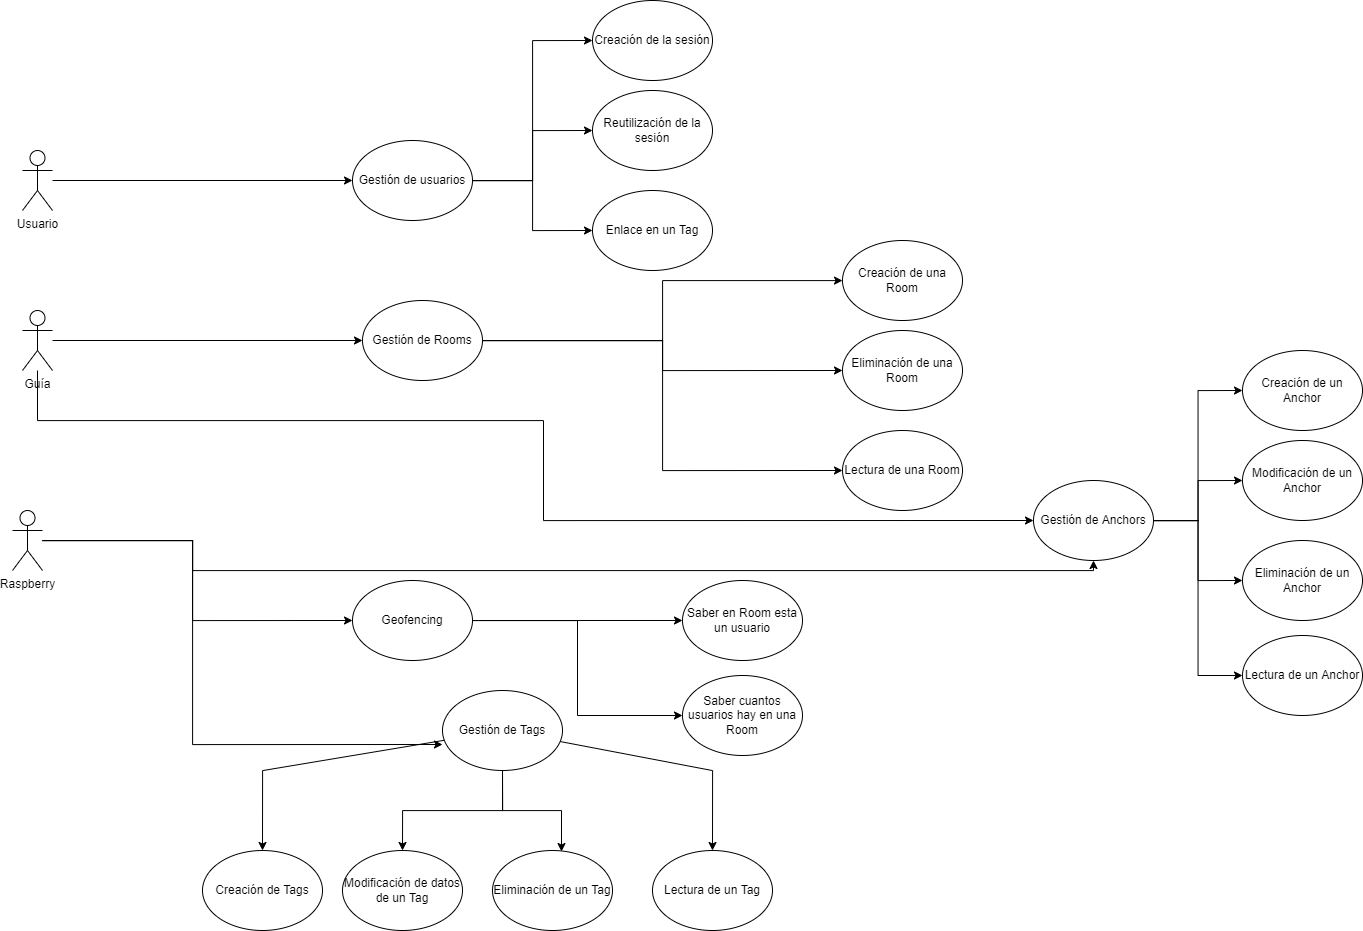
\includegraphics[width=15cm,height=15cm,keepaspectratio]{img/Diagrama General de Casos de uso.drawio (1).png}
    \caption{Diagrama General de Casos de uso.}
    \label{fig:diagrama_general_de_casos_de_uso}
\end{figure}
\FloatBarrier

\begin{table}[H]
    \centering
    \begin{tabular}{p{0.2\textwidth}CGC}
        \hline

        \multicolumn{4}{l}{Caso de uso 1: Gestión de usuarios}\\\hline
        \multirow{2}{*}{Descripción}&\multicolumn{3}{l}{La aplicación debe ser capaz de gestionar
        las sesiones}\\
        &\multicolumn{3}{l}{ de los usuarios.}\\\hline
        \multirow{4}{*}{Requisitos}&\multicolumn{3}{l}{RF 1.1}\\
        \cline{2-4}
        &\multicolumn{3}{l}{RF 1.2}\\
        \cline{2-4}
        &\multicolumn{3}{l}{RF 1.3}\\
        \cline{2-4}
        &\multicolumn{3}{l}{RF 2.4}\\\hline
        
        \multicolumn{1}{l}{Precondiciones}&\multicolumn{3}{l}{La \textit{API} tenga conexión activa con la \textit{bbdd}.}\\\hline
        \multirow{3}{*}{Flujo normal}&\multicolumn{1}{l}{Paso}&\multicolumn{2}{l}{Acción}\\
        \cline{2-4}
        &\multicolumn{1}{l}{1}&\multicolumn{2}{l}{El usuario ejecuta la \textit{WebApp}.}\\
        \cline{2-4}
        &\multicolumn{1}{l}{2}&\multicolumn{2}{l}{El usuario interacciona con el formulario de \textit{Login}.}\\
        \hline
        \multicolumn{1}{l}{Postcondiciones}&\multicolumn{3}{l}{}\\\hline
        \multicolumn{1}{l}{Excepciones}&\multicolumn{3}{l}{Error de \textit{CORS}.}\\\hline
        \multicolumn{1}{l}{Importancia}&\multicolumn{3}{l}{Alta.}\\\hline
        \multicolumn{1}{l}{Urgencia}&\multicolumn{3}{l}{Alta.}\\\hline
        \multicolumn{1}{l}{Comentarios}&\multicolumn{3}{l}{}\\\hline

    \end{tabular}
    \caption{Caso de uso 1: Gestión de usuarios.}
    \label{tab:Caso de uso 1: Gestión de usuarios}
\end{table}

\begin{table}[H]
    \centering
    \begin{tabular}{p{0.2\textwidth}CGC}
        \hline

        \multicolumn{4}{l}{Caso de uso 2: Creación de la sesión}\\\hline
        \multirow{2}{*}{Descripción}&\multicolumn{3}{l}{El usuario debe poder crear una nueva
        sesión con un}\\
        &\multicolumn{3}{l}{alias específico.}\\\hline
        \multirow{3}{*}{Requisitos}&\multicolumn{3}{l}{RF 1.1}\\
        \cline{2-4}
        &\multicolumn{3}{l}{RF 1.3}\\
        \cline{2-4}
        &\multicolumn{3}{l}{RF 2.4}\\
        \hline
        
        \multicolumn{1}{l}{Precondiciones}&\multicolumn{3}{l}{Conexión con la \textit{bbdd}.}\\\hline
        \multirow{6}{*}{Flujo normal}&\multicolumn{1}{l}{Paso}&\multicolumn{2}{l}{Acción}\\
        \cline{2-4}
        &\multicolumn{1}{l}{1}&\multicolumn{2}{l}{El usuario abre la pagina web.}\\
        \cline{2-4}
        &\multicolumn{1}{l}{2}&\multicolumn{2}{l}{Se comprueba que el usuario no existe.}\\
        \cline{2-4}
        &\multicolumn{1}{l}{3}&\multicolumn{2}{l}{Se comprueba que la tag no está enlazada a ningún usuario.}\\
        \cline{2-4}
        &\multicolumn{1}{l}{4}&\multicolumn{2}{l}{Se crea el usuario en la \textit{bbdd}.}\\
        \cline{2-4}
        &\multicolumn{1}{l}{5}&\multicolumn{2}{l}{Se enlaza la \textit{Tag} al usuario.}\\\hline
        \multicolumn{1}{l}{Postcondiciones}&\multicolumn{3}{l}{Se accede al chat.}\\\hline
        \multicolumn{1}{l}{Excepciones}&\multicolumn{3}{l}{Error de \textit{CORS}.}\\\hline
        \multicolumn{1}{l}{Importancia}&\multicolumn{3}{l}{Alta.}\\\hline
        \multicolumn{1}{l}{Urgencia}&\multicolumn{3}{l}{Alta.}\\\hline
        \multicolumn{1}{l}{Comentarios}&\multicolumn{3}{l}{}\\\hline

    \end{tabular}
    \caption{Caso de uso 2: Creación de la sesión.}
    \label{tab:Caso de uso 2: Creación de la sesión}
\end{table}

\begin{table}[H]
    \centering
    \begin{tabular}{p{0.2\textwidth}lGC}
        \hline
        \multicolumn{4}{l}{Caso de uso 3: Reutilización de la sesión}\\\hline
        \multirow{3}{*}{Descripción}&\multicolumn{3}{l}{El usuario debe ser capaz
        de hacer \textit{Login}}\\
        &\multicolumn{3}{l}{si el alias existe en la base de datos}\\
        &\multicolumn{3}{l}{y no está
        enlazado con ninguna \textit{Tag}.}\\\hline
        
        \multirow{3}{*}{Requisitos}&\multicolumn{3}{l}{RF 1.2}\\
        \cline{2-4}
        &\multicolumn{3}{l}{RF 1.3}\\
        \cline{2-4}
        &\multicolumn{3}{l}{RF 2.4}\\
        \hline
        
        \multicolumn{1}{l}{Precondiciones}&\multicolumn{3}{l}{Conexión con la \textit{bbdd}.}\\\hline
        \multirow{5}{*}{Flujo normal}&\multicolumn{1}{l}{Paso}&\multicolumn{2}{l}{Acción}\\
        \cline{2-4}
        &\multicolumn{1}{l}{1}&\multicolumn{2}{l}{El usuario abre la pagina web.}\\
        \cline{2-4}
        &\multicolumn{1}{l}{2}&\multicolumn{2}{l}{Se comprueba que el usuario existe.}\\
        \cline{2-4}
        &\multirow{2}{*}{4}&\multicolumn{2}{l}{Se comprueba que el usuario existe o no}\\
                           &&\multicolumn{2}{l}{existe, sin estar usado.}\\
        \cline{2-4}
        \cline{2-4}
        &\multicolumn{1}{l}{5}&\multicolumn{2}{l}{Se enlaza la \textit{Tag} al usuario.}\\\hline
        \multicolumn{1}{l}{Postcondiciones}&\multicolumn{3}{l}{Se accede a la página chat.}\\\hline
        \multicolumn{1}{l}{Excepciones}&\multicolumn{3}{l}{Error de \textit{CORS}.}\\\hline
        \multicolumn{1}{l}{Importancia}&\multicolumn{3}{l}{Alta.}\\\hline
        \multicolumn{1}{l}{Urgencia}&\multicolumn{3}{l}{Alta.}\\\hline
        \multicolumn{1}{l}{Comentarios}&\multicolumn{3}{l}{}\\\hline

    \end{tabular}
    \caption{Caso de uso 3: Reutilización de la sesión.}
    \label{tab:Caso de uso 3: Reutilización de la sesión}
\end{table}

\begin{table}[H]
    \centering
    \begin{tabular}{ClCC}
        \hline

        \multicolumn{4}{l}{Caso de uso 4: Enlace con un \textit{Tag}}\\\hline
    
        \multirow{2}{*}{Descripción}&\multicolumn{3}{l}{Un usuario debe ser capaz de
        enlazarse con un \textit{Tag}}\\
        &\multicolumn{3}{l}{sino esta enlazado a otro usuario.}\\\hline
        \multirow{1}{*}{Requisitos}&\multicolumn{3}{l}{RF 1.3}\\
        \hline
        
        \multicolumn{1}{l}{Precondiciones}&\multicolumn{3}{l}{Conexión con la \textit{bbdd}.}\\\hline
       
        \multirow{5}{*}{Flujo normal}&\multicolumn{1}{l}{Paso}&\multicolumn{2}{l}{Acción}\\
        \cline{2-4}
        &\multicolumn{1}{l}{1}&\multicolumn{2}{l}{El usuario abre la pagina web.}\\
        \cline{2-4}
        &\multirow{2}{*}{4}&\multicolumn{2}{l}{Se comprueba que el usuario existe o no}\\
                           &&\multicolumn{2}{l}{existe, sin estar usado.}\\
        \cline{2-4}
        &\multirow{2}{*}{3}&\multicolumn{2}{l}{Se comprueba que la \textit{Tag} no está enlazada}\\
                           &&\multicolumn{2}{l}{a ningún usuario.}\\
        \cline{2-4}
        &\multicolumn{1}{l}{5}&\multicolumn{2}{l}{Se enlaza la \textit{Tag} al usuario.}\\\hline
        \multicolumn{1}{l}{Postcondiciones}&\multicolumn{3}{l}{Se enlaza el usuario a la \textit{Tag}.}\\\hline
        \multicolumn{1}{l}{Excepciones}&\multicolumn{3}{l}{Error \textit{CORS}.}\\\hline
        \multicolumn{1}{l}{Importancia}&\multicolumn{3}{l}{Alta.}\\\hline
        \multicolumn{1}{l}{Urgencia}&\multicolumn{3}{l}{Alta.}\\\hline
        \multicolumn{1}{l}{Comentarios}&\multicolumn{3}{l}{}\\\hline

    \end{tabular}
    \caption{Caso de uso 4: Enlace con un \textit{Tag}.}
    \label{tab:Caso de uso 4: Enlace con un Tag}
\end{table}

\begin{table}[H]
    \centering
    \begin{tabular}{p{0.2\textwidth}CGC}
        \hline

        \multicolumn{4}{l}{Caso de uso 5: Gestión de \textit{Tags}}\\\hline
        \multicolumn{1}{l}{Descripción}&\multicolumn{3}{l}{La aplicación debe ser capaz de gestionar
las \textit{Tags}.}\\\hline
        \multirow{4}{*}{Requisitos}&\multicolumn{3}{l}{RF 2.1}\\
        \cline{2-4}
        &\multicolumn{3}{l}{RF 2.2}\\
        \cline{2-4}
        &\multicolumn{3}{l}{RF 2.3}\\
        \cline{2-4}
        &\multicolumn{3}{l}{RF 2.4}\\\hline
        
        \multicolumn{1}{l}{Precondiciones}&\multicolumn{3}{l}{Conexión con la base de datos.}\\\hline
        \multirow{3}{*}{Flujo normal}&\multicolumn{1}{l}{Paso}&\multicolumn{2}{l}{Acción}\\
        \cline{2-4}
        &\multicolumn{1}{l}{1}&\multicolumn{2}{l}{Inicializa el sistema de geolocalización.}\\
        \cline{2-4}
        &\multicolumn{1}{l}{2}&\multicolumn{2}{l}{Se comprueba si la \textit{Tag} existe, sino se añade.}\\\hline

        \multicolumn{1}{l}{Postcondiciones}&\multicolumn{3}{l}{}\\\hline
        \multicolumn{1}{l}{Excepciones}&\multicolumn{3}{l}{Error de conexión de la \textit{bbdd}.}\\\hline
        \multicolumn{1}{l}{Importancia}&\multicolumn{3}{l}{Alta.}\\\hline
        \multicolumn{1}{l}{Urgencia}&\multicolumn{3}{l}{Alta.}\\\hline
        \multicolumn{1}{l}{Comentarios}&\multicolumn{3}{l}{}\\\hline

    \end{tabular}
    \caption{Caso de uso 5: Gestión de \textit{Tags}.}
    \label{tab:Caso de uso 5: Gestión de Tags}
\end{table}

\begin{table}[H]
    \centering
    \begin{tabular}{p{0.2\textwidth}CGC}
        \hline

        \multicolumn{4}{l}{Caso de uso 6: Creación de \textit{Tag}}\\\hline
        \multicolumn{1}{l}{Descripción}&\multicolumn{3}{l}{Las Raspberries deben ser capaces
de crear \textit{Tags}.}\\\hline
        \multirow{1}{*}{Requisitos}&\multicolumn{3}{l}{RF 2.1}\\\hline
        
        \multicolumn{1}{l}{Precondiciones}&\multicolumn{3}{l}{Conexión con la \textit{bbdd}.}\\\hline
        \multirow{4}{*}{Flujo normal}&\multicolumn{1}{l}{Paso}&\multicolumn{2}{l}{Acción}\\
        \cline{2-4}
        &\multicolumn{1}{l}{1}&\multicolumn{2}{l}{Inicializa el sistema de geolocalización.}\\
        \cline{2-4}
        &\multicolumn{1}{l}{2}&\multicolumn{2}{l}{Se comprueba si la \textit{Tag} existe.}\\
        \cline{2-4}
        &\multicolumn{1}{l}{2}&\multicolumn{2}{l}{Si no existe se añade la \textit{Tag}.}\\\hline
        \multicolumn{1}{l}{Postcondiciones}&\multicolumn{3}{l}{Se actualiza la base de datos.}\\\hline
        \multicolumn{1}{l}{Excepciones}&\multicolumn{3}{l}{Error con la \textit{bbdd}.}\\\hline
        \multicolumn{1}{l}{Importancia}&\multicolumn{3}{l}{Alta}\\\hline
        \multicolumn{1}{l}{Urgencia}&\multicolumn{3}{l}{Alta.}\\\hline
        \multicolumn{1}{l}{Comentarios}&\multicolumn{3}{l}{}\\\hline

    \end{tabular}
    \caption{Caso de uso 6: Creación de \textit{Tag}.}
    \label{tab:Caso de uso 6: Creación de Tag}
\end{table}

\begin{table}[H]
    \centering
    \begin{tabular}{p{0.2\textwidth}CGC}
        \hline

        \multicolumn{4}{l}{Caso de uso 7: Modificación de datos de \textit{Tag}}\\\hline
        \multirow{2}{*}{Descripción}&\multicolumn{3}{l}{Las \textit{Raspberries}
        deben ser capaces }\\
        &\multicolumn{3}{l}{de modificar los datos de las \textit{Tags}.}\\\hline
        \multirow{1}{*}{Requisitos}&\multicolumn{3}{l}{RF 2.2 }\\\hline
        \multirow{1}{*}{Precondiciones}&\multicolumn{3}{l}{Conexión con la base de datos.}\\\hline
        
        \multirow{6}{*}{Flujo normal}&\multicolumn{1}{l}{Paso}&\multicolumn{2}{l}{Acción}\\
        \cline{2-4}
        &\multicolumn{1}{l}{1}&\multicolumn{2}{l}{Inicializa el sistema de geolocalización.}\\
        \cline{2-4}
        &\multicolumn{1}{l}{2}&\multicolumn{2}{l}{Se comprueba si la \textit{Tag} existe.}\\
        \cline{2-4}
        &\multicolumn{1}{l}{2}&\multicolumn{2}{l}{Si no existe se añade la \textit{Tag}.}\\
        \cline{2-4}
        &\multicolumn{1}{l}{2}&\multicolumn{2}{l}{Se modifican datos de la \textit{Tag}.}\\\hline
        \multicolumn{1}{l}{Postcondiciones}&\multicolumn{3}{l}{Se actualiza la base de datos.}\\\hline
        \multicolumn{1}{l}{Excepciones}&\multicolumn{3}{l}{Error con la conexión de la \textit{bbdd}.}\\\hline
        \multicolumn{1}{l}{Importancia}&\multicolumn{3}{l}{Alta.}\\\hline
        \multicolumn{1}{l}{Urgencia}&\multicolumn{3}{l}{Alta.}\\\hline
        \multicolumn{1}{l}{Comentarios}&\multicolumn{3}{l}{}\\\hline

    \end{tabular}
    \caption{Caso de uso 7: Modificación de datos de \textit{Tag}.}
    \label{tab:Caso de uso 7: Modificación de datos de Tag}
\end{table}

\begin{table}[H]
    \centering
    \begin{tabular}{p{0.2\textwidth}CGC}
        \hline

        \multicolumn{4}{l}{Caso de uso 8: Eliminación de un \textit{Tag}}\\\hline
        
        \multirow{1}{*}{Descripción}&\multicolumn{3}{l}{ Las \textit{Raspberries} deben ser
capaces de eliminar}\\
        &\multicolumn{3}{l}{un \textit{Tag}.}\\\hline

        \multirow{1}{*}{Requisitos}&\multicolumn{3}{l}{RF 2.3}\\\hline
        
        
        \multicolumn{1}{l}{Precondiciones}&\multicolumn{3}{l}{Conexión con la base de datos}\\\hline
        
        \multirow{5}{*}{Flujo normal}&\multicolumn{1}{l}{Paso}&\multicolumn{2}{l}{Acción}\\
        \cline{2-4}
        &\multicolumn{1}{l}{1}&\multicolumn{2}{l}{Inicializa el sistema de geolocalización.}\\
        \cline{2-4}
        &\multicolumn{1}{l}{2}&\multicolumn{2}{l}{Se comprueba si la \textit{Tag} existe.}\\
        \cline{2-4}
        &\multicolumn{1}{l}{2}&\multicolumn{2}{l}{Si existe se elimina la \textit{Tag}.}\\\hline
        
        \multicolumn{1}{l}{Postcondiciones}&\multicolumn{3}{l}{Se actualiza la base de datos.}\\\hline
        
        \multicolumn{1}{l}{Excepciones}&\multicolumn{3}{l}{Error con la conexión de la \textit{bbdd}.}\\\hline
        
        \multicolumn{1}{l}{Importancia}&\multicolumn{3}{l}{Alta.}\\\hline
        
        \multicolumn{1}{l}{Urgencia}&\multicolumn{3}{l}{Alta.}\\\hline
        
        \multicolumn{1}{l}{Comentarios}&\multicolumn{3}{l}{}\\\hline

    \end{tabular}
    \caption{Caso de uso 8: Eliminación de un \textit{Tag}.}
    \label{tab:Caso de uso 8: Eliminación de un Tag}
\end{table}

\begin{table}[H]
    \centering
    \begin{tabular}{p{0.2\textwidth}CGC}
        \hline

        \multicolumn{4}{l}{Caso de uso 9: Lectura de \textit{Tag}}\\\hline
        
        \multirow{2}{*}{Descripción}&\multicolumn{3}{l}{La aplicación debe ser capaz de
        leer un }\\
        &\multicolumn{3}{l}{determinado \textit{Tag}.}\\\hline
        
        \multirow{1}{*}{Requisitos}&\multicolumn{3}{l}{RF 2.4}\\\hline
        
        
        \multicolumn{1}{l}{Precondiciones}&\multicolumn{3}{l}{Debe existir una conexión con la \textit{bbdd}.}\\\hline
        \multirow{5}{*}{Flujo normal}&\multicolumn{1}{l}{Paso}&\multicolumn{2}{l}{Acción}\\
        \cline{2-4}
        &\multicolumn{1}{l}{1}&\multicolumn{2}{l}{Inicializa el sistema de geolocalización.}\\
        \cline{2-4}
        &\multicolumn{1}{l}{2}&\multicolumn{2}{l}{Se lee la \textit{Tag}.}\\
    
        
        \multicolumn{1}{l}{Postcondiciones}&\multicolumn{3}{l}{}\\\hline
        \multicolumn{1}{l}{Excepciones}&\multicolumn{3}{l}{Error con la conexión de la \textit{bbdd}.}\\\hline
        \multicolumn{1}{l}{Importancia}&\multicolumn{3}{l}{Alta.}\\\hline
        \multicolumn{1}{l}{Urgencia}&\multicolumn{3}{l}{Alta.}\\\hline
        \multicolumn{1}{l}{Comentarios}&\multicolumn{3}{l}{}\\\hline

    \end{tabular}
    \caption{Caso de uso 9: Lectura de \textit{Tag}.}
    \label{tab:Caso de uso 9: Lectura de Tag}
\end{table}

\begin{table}[H]
    \centering
    \begin{tabular}{p{0.2\textwidth}CGC}
        \hline

        \multicolumn{4}{l}{Caso de uso 10: Gestión de \textit{Anchors}.}\\\hline
        \multicolumn{1}{l}{Descripción}&\multicolumn{3}{l}{La aplicación debe ser capaz de
        gestionar las \textit{Anchors}.}\\\hline
        \multirow{3}{*}{Requisitos}&\multicolumn{3}{l}{RF 4.1}\\
        \cline{2-4}
        &\multicolumn{3}{l}{RF 4.2}\\
        \cline{2-4}
        &\multicolumn{3}{l}{RF 4.3}\\\hline
        
        \multicolumn{1}{l}{Precondiciones}&\multicolumn{3}{l}{Conexión con la \textit{bbdd}.}\\\hline
        \multirow{3}{*}{Flujo normal}&\multicolumn{1}{l}{Paso}&\multicolumn{2}{l}{Acción}\\
        \cline{2-4}
        &\multicolumn{1}{l}{1}&\multicolumn{2}{l}{Inicializa el sistema de geolocalización}\\
        \cline{2-4}
        &\multicolumn{1}{l}{2}&\multicolumn{2}{l}{Se comprueba si el \textit{anchor} existe, sino se añade}\\\hline

        \multicolumn{1}{l}{Postcondiciones}&\multicolumn{3}{l}{}\\\hline
        \multicolumn{1}{l}{Excepciones}&\multicolumn{3}{l}{Error de conexión de la \textit{bbdd}.}\\\hline
        \multicolumn{1}{l}{Importancia}&\multicolumn{3}{l}{Alta.}\\\hline
        \multicolumn{1}{l}{Urgencia}&\multicolumn{3}{l}{Alta.}\\\hline
        \multicolumn{1}{l}{Comentarios}&\multicolumn{3}{l}{}\\\hline
    \end{tabular}
    \caption{Caso de uso 10: Gestión de \textit{Anchors}.}
    \label{tab:Caso de uso 10: Gestión de Anchors}
\end{table}

\begin{table}[H]
    \centering
    \begin{tabular}{p{0.2\textwidth}CGC}
        \hline

        \multicolumn{4}{l}{Caso de uso 11: Creación de \textit{Anchor}}\\\hline
        \multicolumn{1}{l}{Descripción}&\multicolumn{3}{l}{Las \textit{Raspberries} deben ser
        capaces de crear un Anchor.}\\\hline
        \multirow{2}{*}{Requisitos}&\multicolumn{3}{l}{RF 3.1}\\
        \cline{2-4}
        &\multicolumn{3}{l}{RF 3.4}\\\hline
        
        \multicolumn{1}{l}{Precondiciones}&\multicolumn{3}{l}{Tener una conexión con la \textit{bbdd}.}\\\hline
        \multirow{4}{*}{Flujo normal}&\multicolumn{1}{l}{Paso}&\multicolumn{2}{l}{Acción}\\
        \cline{2-4}
        &\multicolumn{1}{l}{1}&\multicolumn{2}{l}{Inicializa el sistema de geolocalización.}\\
        \cline{2-4}
        &\multicolumn{1}{l}{2}&\multicolumn{2}{l}{Se comprueba si el \textit{Anchor} existe.}\\
        \cline{2-4}
        &\multicolumn{1}{l}{2}&\multicolumn{2}{l}{Si no existe se añade el \textit{Anchor}.}\\\hline
        \multicolumn{1}{l}{Postcondiciones}&\multicolumn{3}{l}{Se actualiza la base de datos.}\\\hline
        \multicolumn{1}{l}{Excepciones}&\multicolumn{3}{l}{Error con la conexión de la \textit{bbdd}.}\\\hline
        \multicolumn{1}{l}{Importancia}&\multicolumn{3}{l}{Alta.}\\\hline
        \multicolumn{1}{l}{Urgencia}&\multicolumn{3}{l}{Alta.}\\\hline
        \multicolumn{1}{l}{Comentarios}&\multicolumn{3}{l}{}\\\hline

    \end{tabular}
    \caption{Caso de uso 11: Creación de \textit{Anchor}.}
    \label{tab:Caso de uso 11: Creación de Anchor}
\end{table}

\begin{table}[H]
    \centering
    \begin{tabular}{p{0.2\textwidth}CGC}
        \hline

        \multicolumn{4}{l}{Caso de uso 12: Modificación de datos de \textit{Anchor}}\\\hline
        \multirow{2}{*}{Descripción}&\multicolumn{3}{l}{Las \textit{Raspberries} o los usuarios deben ser }\\
        &\multicolumn{3}{l}{ capaces de modificar datos en los
        \textit{Anchors}.}\\\hline
        \multirow{2}{*}{Requisitos}&\multicolumn{3}{l}{RF 3.2}\\
        \cline{2-4}
        &\multicolumn{3}{l}{RF 3.4}\\\hline
        
        \multicolumn{1}{l}{Precondiciones}&\multicolumn{3}{l}{Conexión con la \textit{bbdd}.}\\\hline
        \multirow{4}{*}{Flujo normal}&\multicolumn{1}{l}{Paso}&\multicolumn{2}{l}{Acción}\\
        \cline{2-4}
        &\multicolumn{1}{l}{1}&\multicolumn{2}{l}{Inicializa el sistema de geolocalización.}\\
        \cline{2-4}
        &\multicolumn{1}{l}{2}&\multicolumn{2}{l}{Se comprueba si el \textit{Anchor} existe.}\\
        \cline{2-4}
        &\multicolumn{1}{l}{2}&\multicolumn{2}{l}{Si existe, se modifican los datos del \textit{Anchor}.}\\\hline
        \multicolumn{1}{l}{Postcondiciones}&\multicolumn{3}{l}{Se actualiza la base de datos.}\\\hline
        \multicolumn{1}{l}{Excepciones}&\multicolumn{3}{l}{Error con la conexión con la \textit{bbdd}.}\\\hline
        \multicolumn{1}{l}{Importancia}&\multicolumn{3}{l}{Alta.}\\\hline
        \multicolumn{1}{l}{Urgencia}&\multicolumn{3}{l}{Alta.}\\\hline
        \multicolumn{1}{l}{Comentarios}&\multicolumn{3}{l}{}\\\hline

    \end{tabular}
    \caption{Caso de uso 12: Modificación de datos de \textit{Anchor}.}
    \label{tab:Caso de uso 12: Modificación de datos de Anchor}
\end{table}

\begin{table}[H]
    \centering
    \begin{tabular}{p{0.2\textwidth}CGC}
        \hline

        \multicolumn{4}{l}{Caso de uso 13: Eliminación de un \textit{Anchor}}\\\hline
        \multicolumn{1}{l}{Descripción}&\multicolumn{3}{l}{Las Raspberries deben
ser capaces de eliminar un \textit{Anchor}.}\\\hline
        \multirow{1}{*}{Requisitos}&\multicolumn{3}{l}{RF 3.3}\\\hline
        
        \multicolumn{1}{l}{Precondiciones}&\multicolumn{3}{l}{Conexión con la \textit{bbdd}.}\\\hline
        \multirow{4}{*}{Flujo normal}&\multicolumn{1}{l}{Paso}&\multicolumn{2}{l}{Acción}\\
        \cline{2-4}
        &\multicolumn{1}{l}{1}&\multicolumn{2}{l}{Inicializa el sistema de geolocalización.}\\
        \cline{2-4}
        &\multicolumn{1}{l}{2}&\multicolumn{2}{l}{Se comprueba si el \textit{Anchor} existe.}\\
        \cline{2-4}
        &\multicolumn{1}{l}{2}&\multicolumn{2}{l}{Si existe, se elimina el \textit{Anchor}.}\\\hline
        \multicolumn{1}{l}{Postcondiciones}&\multicolumn{3}{l}{Se actualiza la base de datos.}\\\hline
        \multicolumn{1}{l}{Excepciones}&\multicolumn{3}{l}{Error con la conexión de la \textit{bbdd}.}\\\hline
        \multicolumn{1}{l}{Importancia}&\multicolumn{3}{l}{Alta}\\\hline
        \multicolumn{1}{l}{Urgencia}&\multicolumn{3}{l}{Alta}\\\hline
        \multicolumn{1}{l}{Comentarios}&\multicolumn{3}{l}{}\\\hline

    \end{tabular}
    \caption{Caso de uso 13: Eliminación de un \textit{Anchor}.}
    \label{tab:Caso de uso 13: Eliminación de un Anchor}
\end{table}

\begin{table}[H]
    \centering
    \begin{tabular}{p{0.2\textwidth}CGC}
        \hline

        \multicolumn{4}{l}{Caso de uso 14: Lectura de \textit{Anchor}}\\\hline
        \multicolumn{1}{l}{Descripción}&\multicolumn{3}{l}{ La aplicación debe ser capaz
de leer un \textit{Anchor}.}\\\hline
        \multirow{1}{*}{Requisitos}&\multicolumn{3}{l}{RF 3.4}\\\hline
     
        
        \multicolumn{1}{l}{Precondiciones}&\multicolumn{3}{l}{Conexión con la \textit{bbdd}.}\\\hline
        \multirow{3}{*}{Flujo normal}&\multicolumn{1}{l}{Paso}&\multicolumn{2}{l}{Acción}\\
        \cline{2-4}
        &\multicolumn{1}{l}{1}&\multicolumn{2}{l}{Inicializa el sistema de geolocalización.}\\
        \cline{2-4}
        &\multicolumn{1}{l}{2}&\multicolumn{2}{l}{Se comprueba si el \textit{Anchor} existe.}\\
        \multicolumn{1}{l}{Postcondiciones}&\multicolumn{3}{l}{Se leen datos de la \textit{bbdd}.}\\\hline
        \multicolumn{1}{l}{Excepciones}&\multicolumn{3}{l}{Error con la conexión de la \textit{bbdd}.}\\\hline
        \multicolumn{1}{l}{Importancia}&\multicolumn{3}{l}{Alta}\\\hline
        \multicolumn{1}{l}{Urgencia}&\multicolumn{3}{l}{Alta}\\\hline
        \multicolumn{1}{l}{Comentarios}&\multicolumn{3}{l}{}\\\hline

    \end{tabular}
    \caption{Caso de uso 14: Lectura de \textit{Anchor}.}
    \label{tab:Caso de uso 14: Lectura de Anchor}
\end{table}

\begin{table}[H]
    \centering
    \begin{tabular}{p{0.2\textwidth}lGC}
        \hline

        \multicolumn{4}{l}{Caso de uso 15: Gestión de \textit{Rooms}}\\\hline
        \multirow{2}{*}{Descripción}&\multicolumn{3}{l}{La aplicación debe ser capaz de gestionar }\\
        &\multicolumn{3}{l}{ las \textit{Rooms}.}\\\hline
        \multirow{3}{*}{Requisitos}&\multicolumn{3}{l}{RF 4.1}\\
        \cline{2-4}
        &\multicolumn{3}{l}{RF 4.2}\\
        \cline{2-4}
        &\multicolumn{3}{l}{RF 4.3}\\\hline
        
        \multicolumn{1}{l}{Precondiciones}&\multicolumn{3}{l}{Conexión con la base de datos.}\\\hline
        \multirow{4}{*}{Flujo normal}&\multicolumn{1}{l}{Paso}&\multicolumn{2}{l}{Acción}\\
        \cline{2-4}
        &\multicolumn{1}{l}{1}&\multicolumn{2}{l}{Se \textit{logea} un guia desde la \textit{webapp}.}\\
        \cline{2-4}
        &\multicolumn{1}{l}{2}&\multicolumn{2}{l}{Desde el \textit{chat} accede al mapa.}\\
        \cline{2-4}
        &\multicolumn{1}{l}{3}&\multicolumn{2}{l}{Desde el mapa accede a \textit{editarMapa}.}\\\hline
        \multicolumn{1}{l}{Postcondiciones}&\multicolumn{3}{l}{}\\\hline
        \multicolumn{1}{l}{Excepciones}&\multicolumn{3}{l}{Error con la conexión de la \textit{bbdd}.}\\\hline
        \multicolumn{1}{l}{Importancia}&\multicolumn{3}{l}{Alta.}\\\hline
        \multicolumn{1}{l}{Urgencia}&\multicolumn{3}{l}{Alta.}\\\hline
        \multicolumn{1}{l}{Comentarios}&\multicolumn{3}{l}{}\\\hline

    \end{tabular}
    \caption{Caso de uso 15: Gestión de \textit{Rooms}.}
    \label{tab:Caso de uso 15: Gestión de Rooms}
\end{table}

\begin{table}[H]
    \centering
    \begin{tabular}{p{0.2\textwidth}CGC}
        \hline

        \multicolumn{4}{l}{Caso de uso 16: Creación de una \textit{Room}}\\\hline
        \multicolumn{1}{l}{Descripción}&\multicolumn{3}{l}{ Un guía debe ser capaz de
crear una \textit{Room}.}\\\hline
        \multirow{1}{*}{Requisitos}&\multicolumn{3}{l}{RF 4.1}\\\hline

        
        \multicolumn{1}{l}{Precondiciones}&\multicolumn{3}{l}{Conexión con la \textit{bbdd}.}\\\hline
        \multirow{6}{*}{Flujo normal}&\multicolumn{1}{l}{Paso}&\multicolumn{2}{l}{Acción}\\
        \cline{2-4}
        &\multicolumn{1}{l}{1}&\multicolumn{2}{l}{Se logea un guia desde la webapp.}\\
        \cline{2-4}
        &\multicolumn{1}{l}{2}&\multicolumn{2}{l}{Desde el chat accede al mapa.}\\
        \cline{2-4}
        &\multicolumn{1}{l}{3}&\multicolumn{2}{l}{Desde el mapa accede a \textit{editarMapa}.}\\
        \cline{2-4}
        &\multicolumn{1}{l}{4}&\multicolumn{2}{l}{Se dibuja la \textit{Room}.}\\
        \cline{2-4}
        &\multicolumn{1}{l}{5}&\multicolumn{2}{l}{Se guarda la \textit{Room}.}\\\hline
        \multicolumn{1}{l}{Postcondiciones}&\multicolumn{3}{l}{Se crea la \textit{Room} en la \textit{bbdd}.}\\\hline
        \multicolumn{1}{l}{Excepciones}&\multicolumn{3}{l}{Error con la conexión de la \textit{bbdd}.}\\\hline
        \multicolumn{1}{l}{Importancia}&\multicolumn{3}{l}{Alta.}\\\hline
        \multicolumn{1}{l}{Urgencia}&\multicolumn{3}{l}{Alta.}\\\hline
        \multicolumn{1}{l}{Comentarios}&\multicolumn{3}{l}{}\\\hline

    \end{tabular}
    \caption{Caso de uso 16: Creación de una \textit{Room}.}
    \label{tab:Caso de uso 16: Creación de una Room}
\end{table}

\begin{table}[H]
    \centering
    \begin{tabular}{p{0.2\textwidth}CGC}
        \hline

        \multicolumn{4}{l}{Caso de uso 17: Eliminación de una \textit{Room}}\\\hline
        \multicolumn{1}{l}{Descripción}&\multicolumn{3}{l}{ Un guía debe ser capaz de eliminar una \textit{Room}.}\\\hline
        \multirow{1}{*}{Requisitos}&\multicolumn{3}{l}{RF 4.2}\\\hline

        
        \multicolumn{1}{l}{Precondiciones}&\multicolumn{3}{l}{Conexión con la \textit{bbdd}.}\\\hline
        \multirow{6}{*}{Flujo normal}&\multicolumn{1}{l}{Paso}&\multicolumn{2}{l}{Acción}\\
        \cline{2-4}
        &\multicolumn{1}{l}{1}&\multicolumn{2}{l}{Se \textit{logea} un guia desde la \textit{webapp}.}\\
        \cline{2-4}
        &\multicolumn{1}{l}{2}&\multicolumn{2}{l}{Desde el chat accede al mapa.}\\
        \cline{2-4}
        &\multicolumn{1}{l}{3}&\multicolumn{2}{l}{Desde el mapa accede a \textit{editarMapa}.}\\
        \cline{2-4}
        &\multicolumn{1}{l}{4}&\multicolumn{2}{l}{Se elige la \textit{Room} a eliminar.}\\
        \cline{2-4}
        &\multicolumn{1}{l}{5}&\multicolumn{2}{l}{Se pulsa el botón eliminar.}\\\hline
        \multicolumn{1}{l}{Postcondiciones}&\multicolumn{3}{l}{Se eliminar una \textit{Room} de la \textit{bbdd}.}\\\hline
        \multicolumn{1}{l}{Excepciones}&\multicolumn{3}{l}{Error con la conexión de la \textit{bbdd}.}\\\hline
        \multicolumn{1}{l}{Importancia}&\multicolumn{3}{l}{Alta.}\\\hline
        \multicolumn{1}{l}{Urgencia}&\multicolumn{3}{l}{Alta.}\\\hline
        \multicolumn{1}{l}{Comentarios}&\multicolumn{3}{l}{}\\\hline

    \end{tabular}
    \caption{Caso de uso 17: Eliminación de una \textit{Room}.}
    \label{tab:Caso de uso 17: Eliminación de una Room}
\end{table}

\begin{table}[H]
    \centering
    \begin{tabular}{p{0.2\textwidth}CGC}
        \hline

        \multicolumn{4}{l}{Caso de uso 18: Lectura de una \textit{Room}}\\\hline
        \multicolumn{1}{l}{Descripción}&\multicolumn{3}{l}{La aplicación debe ser capaz
de eliminar una \textit{Room}.}\\\hline
        \multirow{1}{*}{Requisitos}&\multicolumn{3}{l}{4.3}\\\hline
        
        \multicolumn{1}{l}{Precondiciones}&\multicolumn{3}{l}{Conexión con la base de datos.}\\\hline
        \multirow{5}{*}{Flujo normal}&\multicolumn{1}{l}{Paso}&\multicolumn{2}{l}{Acción}\\
        \cline{2-4}
        &\multicolumn{1}{l}{1}&\multicolumn{2}{l}{Se \textit{logea} un guia desde la \textit{webapp}.}\\
        \cline{2-4}
        &\multicolumn{1}{l}{2}&\multicolumn{2}{l}{Desde el \textit{chat} accede al mapa.}\\
        \cline{2-4}
        &\multicolumn{1}{l}{3}&\multicolumn{2}{l}{Desde el mapa accede a \textit{editarMapa}.}\\
        \cline{2-4}
        &\multicolumn{1}{l}{4}&\multicolumn{2}{l}{Se leen las \textit{Rooms} desde la \textit{bbdd}.}\\\hline
        \multicolumn{1}{l}{Postcondiciones}&\multicolumn{3}{l}{Se devuelve el objeto \textit{Room}.}\\\hline
        \multicolumn{1}{l}{Excepciones}&\multicolumn{3}{l}{Error con la conexión de la \textit{bbdd}.}\\\hline
        \multicolumn{1}{l}{Importancia}&\multicolumn{3}{l}{Alta.}\\\hline
        \multicolumn{1}{l}{Urgencia}&\multicolumn{3}{l}{Alta.}\\\hline
        \multicolumn{1}{l}{Comentarios}&\multicolumn{3}{l}{}\\\hline

    \end{tabular}
    \caption{Caso de uso 18: Lectura de una \textit{Room}.}
    \label{tab:table-total-costs}
\end{table}

\begin{table}[H]
    \centering
    \begin{tabular}{p{0.2\textwidth}CGC}
        \hline

        \multicolumn{4}{l}{Caso de uso 19: \textit{Geofencing}}\\\hline
        \multirow{2}{*}{Descripción}&\multicolumn{3}{l}{La aplicación debe ser capaz de gestionar }\\
        &\multicolumn{3}{l}{ el geofencing de \textit{Tags} y \textit{Rooms}.}\\\hline        \multirow{2}{*}{Requisitos}&\multicolumn{3}{l}{RF 5.1}\\
        \cline{2-4}
        &\multicolumn{3}{l}{RF 5.2}\\\hline
        
        \multicolumn{1}{l}{Precondiciones}&\multicolumn{3}{l}{\textit{Tile38} activada y con datos.}\\\hline
        \multirow{5}{*}{Flujo normal}&\multicolumn{1}{l}{Paso}&\multicolumn{2}{l}{Acción}\\
        \cline{2-4}
        &\multicolumn{1}{l}{1}&\multicolumn{2}{l}{El usuario se \textit{logea}.}\\
        \cline{2-4}
        &\multicolumn{1}{l}{2}&\multicolumn{2}{l}{Se crea una instancia en \textit{Tile38}}\\
        \cline{2-4}
        &\multicolumn{1}{l}{3}&\multicolumn{2}{l}{Se triangula con la \textit{Room}, también guardada.}\\
        \cline{2-4}
        &\multicolumn{1}{l}{4}&\multicolumn{2}{l}{Se devuelve el dato requerido.}\\\hline
        \multicolumn{1}{l}{Postcondiciones}&\multicolumn{3}{l}{}\\\hline
        \multicolumn{1}{l}{Excepciones}&\multicolumn{3}{l}{El dato que se requiere no existe en \textit{Tile38}.}\\\hline
        \multicolumn{1}{l}{Importancia}&\multicolumn{3}{l}{Normal.}\\\hline
        \multicolumn{1}{l}{Urgencia}&\multicolumn{3}{l}{Normal.}\\\hline
        \multicolumn{1}{l}{Comentarios}&\multicolumn{3}{l}{}\\\hline

    \end{tabular}
    \caption{Caso de uso 19: \textit{Geofencing}.}
    \label{tab:Caso de uso 19: Geofencing}
\end{table}

\begin{table}[H]
    \centering
    \begin{tabular}{p{0.2\textwidth}lGC}
        \hline

        \multicolumn{4}{l}{Caso de uso 20: Saber en que \textit{Room} está un usuario.}\\\hline
        \multirow{2}{*}{Descripción}&\multicolumn{3}{l}{ La aplicación debe ser capaz de }\\
        &\multicolumn{3}{l}{determinar en que \textit{Room} está un usuario.}\\\hline           \multirow{1}{*}{Requisitos}&\multicolumn{3}{l}{RF 5.1}\\\hline
        
        \multicolumn{1}{l}{Precondiciones}&\multicolumn{3}{l}{Tile38 activada y con datos.}\\\hline
        \multirow{4}{*}{Flujo normal}&\multicolumn{1}{l}{Paso}&\multicolumn{2}{l}{Acción}\\
        \cline{2-4}
        &\multicolumn{1}{l}{1}&\multicolumn{2}{l}{El guía se \textit{logea}.}\\
        \cline{2-4}
        &\multicolumn{1}{l}{2}&\multicolumn{2}{l}{Se accede al \textit{chat}}\\
        \cline{2-4}
        &\multirow{2}{*}{3}&\multicolumn{2}{l}{Si un usuario entra a una \textit{Room} se le }\\
                           &&\multicolumn{2}{l}{proporciona contenido personalizado de la \textit{Room}.}\\\hline
        \multicolumn{1}{l}{Postcondiciones}&\multicolumn{3}{l}{Se obtiene la \textit{Room} en la que esta la \textit{Tag}.}\\\hline
        \multicolumn{1}{l}{Excepciones}&\multicolumn{3}{l}{El dato que se requiere no existe en \textit{Tile38}.}\\\hline
        \multicolumn{1}{l}{Importancia}&\multicolumn{3}{l}{Normal}\\\hline
        \multicolumn{1}{l}{Urgencia}&\multicolumn{3}{l}{Normal}\\\hline
        \multicolumn{1}{l}{Comentarios}&\multicolumn{3}{l}{}\\\hline

    \end{tabular}
    \caption{Caso de uso 20: Saber en que \textit{Room} está un usuario.}
    \label{tab:Caso de uso 20: Saber en que Room está un usuario}
\end{table}

\begin{table}[H]
    \centering
    \begin{tabular}{p{0.2\textwidth}CGC}
        \hline

        \multicolumn{4}{l}{Caso de uso 21: Saber cuantos usuarios están en una \textit{Room}.}\\\hline
        \multirow{2}{*}{Descripción}&\multicolumn{3}{l}{ La aplicación debe ser capaz de saber }\\
        &\multicolumn{3}{l}{cuantos usuarios para hay en una \textit{Room}.}\\\hline           \multirow{1}{*}{Requisitos}&\multicolumn{3}{l}{RF 5.2}\\\hline
        
        \multicolumn{1}{l}{Precondiciones}&\multicolumn{3}{l}{\textit{Tile38} activada y con datos.}\\\hline
        \multirow{4}{*}{Flujo normal}&\multicolumn{1}{l}{Paso}&\multicolumn{2}{l}{Acción}\\
        \cline{2-4}
        &\multicolumn{1}{l}{1}&\multicolumn{2}{l}{El guía se \textit{logea}.}\\
        \cline{2-4}
        &\multicolumn{1}{l}{2}&\multicolumn{2}{l}{Se accede al mapa}\\
        \cline{2-4}
        &\multicolumn{1}{l}{3}&\multicolumn{2}{l}{En el \textit{sidebar} se ven las \textit{Rooms} con los usuarios.}\\\hline
        \multicolumn{1}{l}{Postcondiciones}&\multicolumn{3}{l}{Se obtiene el numero de \textit{Tags} en una \textit{Room}.}\\\hline
        \multicolumn{1}{l}{Excepciones}&\multicolumn{3}{l}{El dato que se requiere no existe en \textit{Tile38}.}\\\hline
        \multicolumn{1}{l}{Importancia}&\multicolumn{3}{l}{Normal.}\\\hline
        \multicolumn{1}{l}{Urgencia}&\multicolumn{3}{l}{Normal.}\\\hline
        \multicolumn{1}{l}{Comentarios}&\multicolumn{3}{l}{}\\\hline

    \end{tabular}
    \caption{Caso de uso 21: Saber cuantos usuarios están en una \textit{Room}.}
    \label{tab:Caso de uso 21: Saber cuantos usuarios están en una Room}
\end{table}


